\documentclass[journal]{IEEEtran}
\usepackage{iftex}
\ifPDFTeX
  \usepackage[utf8]{inputenc}
  \usepackage[T1]{fontenc}
\else
  \usepackage{fontspec}
  \setmainfont{texgyretermes}[Extension=.otf, UprightFont=*-regular, BoldFont=*-bold,
    ItalicFont=*-italic, BoldItalicFont=*-bolditalic]
\fi
\usepackage[spanish,es-tabla,es-nodecimaldot,es-noshorthands]{babel}
\usepackage{amsmath,amssymb}
\usepackage{graphicx}
\usepackage{booktabs}
\usepackage{url}
\usepackage{cite}
\graphicspath{{figuras/}}

\begin{document}

\title{Clasificación de Imágenes de Futbolistas mediante un Ensemble de CLIP y ConvNeXt con Transfer Learning}

\author{Carlos~Flores, Leonardo~de~Casanova y~Miguel~Ángel~Mori%
\thanks{Los autores pertenecen a la Universidad de Ingeniería y Tecnología (UTEC), Lima, Perú.}%
\thanks{Código y notebooks: \protect\url{https://github.com/Los-1000/machine-learning-final}.}}

\markboth{Proyecto Final de Machine Learning, noviembre~2026}%
{Flores \MakeLowercase{\textit{et al.}}: Clasificación de imágenes de futbolistas}

\maketitle

\begin{abstract}
Una compañía de publicidad deportiva necesita identificar automáticamente qué futbolista aparece en una imagen. Se usa el conjunto \textit{Golden Foot}, con cerca de 7\,200 fotografías de 22 futbolistas tomadas de internet en condiciones muy heterogéneas. Se propone un ensemble de dos modelos preentrenados y complementarios. El primero es el codificador visual de CLIP ViT-L/14, usado como extractor de características con una regresión logística multinomial encima. El segundo es una red ConvNeXt-Small reentrenada por completo con aumento de datos. Las probabilidades de ambos se combinan mediante \textit{soft voting}, con un peso elegido en validación. En un conjunto de prueba estratificado de 1\,077 imágenes, el ensemble obtiene un \textit{recall} macro de 0.968 y un F1 macro de 0.968, lo que supera el requisito de 0.9 y a cada modelo por separado.
\end{abstract}

\begin{IEEEkeywords}
Clasificación de imágenes, transfer learning, CLIP, ConvNeXt, ensemble learning, soft voting, reconocimiento de personas.
\end{IEEEkeywords}

\section{Introducción}
\IEEEPARstart{E}{n} el sector de la publicidad deportiva es frecuente tener que etiquetar grandes volúmenes de fotografías según el jugador que aparece en ellas. Hacerlo a mano es costoso y propenso a errores. Las redes neuronales profundas permiten automatizar esta tarea, pero entrenarlas desde cero exige muchos datos por clase. En este problema se dispone de solo unas 330 imágenes por jugador, tomadas en escenarios muy variados.

El \textit{transfer learning} resuelve esta limitación: reutiliza modelos preentrenados en millones de imágenes y los adapta al problema con pocos datos.

El objetivo de este trabajo es construir un modelo en conjunto (\textit{ensemble}) que clasifique las imágenes de 22 futbolistas con un \textit{recall} y un F1-score mayores a 0.9.

\section{Descripción de los datos}
El conjunto \textit{Golden Foot Football Players Image Dataset}~\cite{dataset} se organiza en un directorio por jugador. Un archivo CSV con las columnas \texttt{folder\_name} y \texttt{filename} relaciona cada imagen con el nombre del futbolista. Incluye 22 jugadores, entre ellos Messi, Cristiano Ronaldo, Pelé, Maradona, Modric y Salah.

La Fig.~\ref{fig:clases} muestra cuántas imágenes hay por clase: entre 239 y 350. El desbalance es leve (razón 1.46). Las clases con menos imágenes son Pelé, Nedved y Ronaldo Nazário, jugadores retirados de quienes existen menos fotografías recientes.

\begin{figure}[!t]
\centering
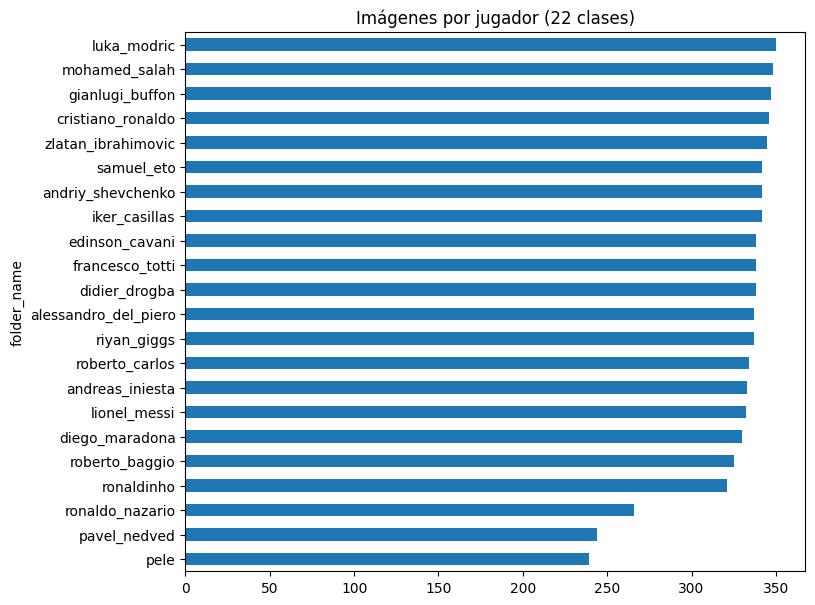
\includegraphics[width=0.85\columnwidth]{distribucion_clases.png}
\caption{Número de imágenes por futbolista después de la limpieza.}
\label{fig:clases}
\end{figure}

Las imágenes son muy heterogéneas (Fig.~\ref{fig:muestra}):
\begin{itemize}
\item \textbf{Tamaño:} su resolución va de unos 140~px a más de 3\,000~px de lado.
\item \textbf{Encuadre:} aparecen primeros planos, el jugador de cuerpo entero en el campo y fotos con varias personas.
\item \textbf{Época:} hay fotografías antiguas en blanco y negro y fotos del jugador en distintas etapas de su vida (en activo, retirado o como entrenador).
\end{itemize}

\begin{figure*}[!t]
\centering
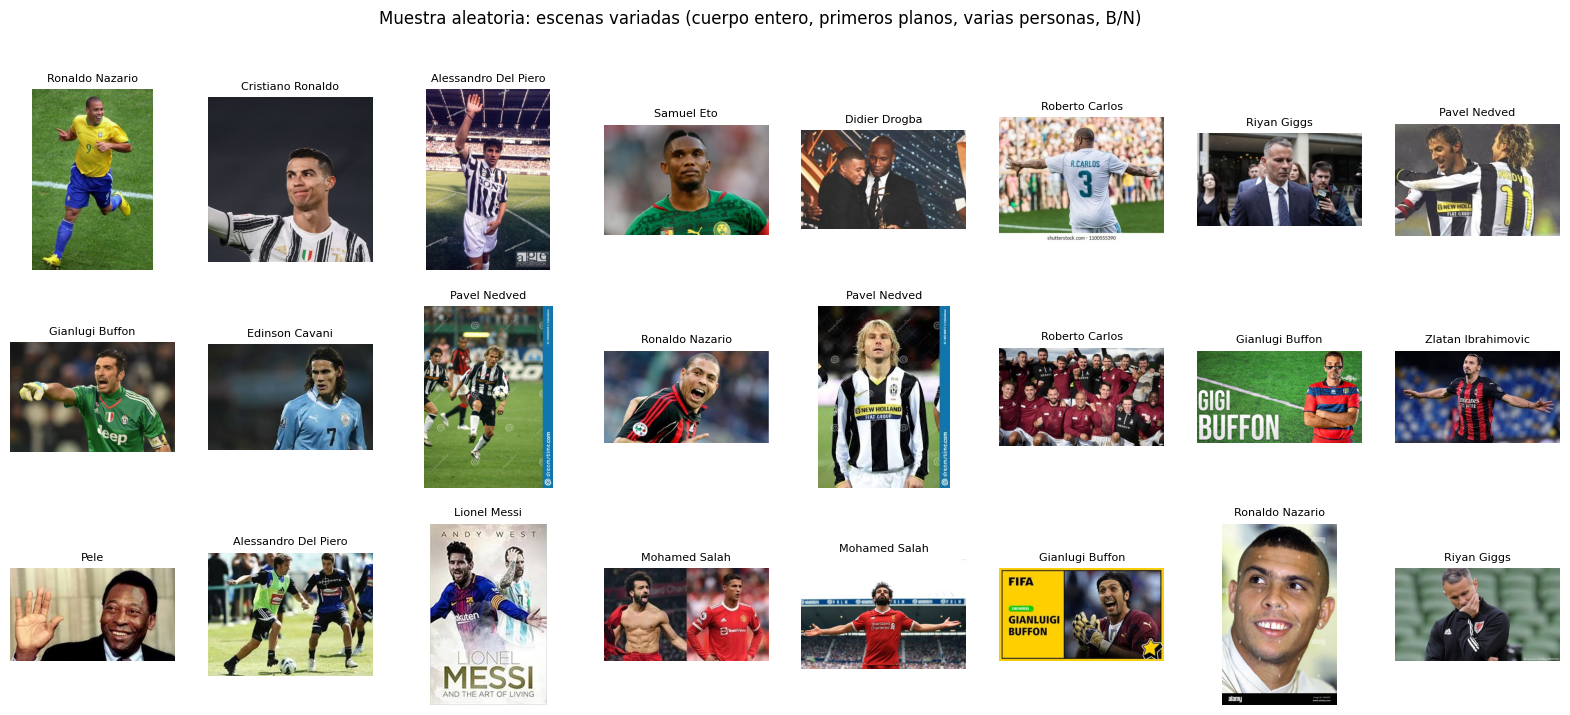
\includegraphics[width=0.95\textwidth]{muestra.png}
\caption{Muestra aleatoria del conjunto de datos. Se observan distintas escalas, poses, varias personas por imagen y fotografías en blanco y negro.}
\label{fig:muestra}
\end{figure*}

\subsection{Limpieza}
Se aplicaron tres pasos de limpieza:
\begin{enumerate}
\item Se descartó una fila vacía del CSV y se verificó que existiera cada archivo (7\,188 imágenes).
\item Se calculó el hash MD5 de cada archivo. Siete imágenes idénticas aparecían en carpetas de dos jugadores distintos y se eliminaron, porque su etiqueta es contradictoria. Los duplicados exactos se conservaron una sola vez, para evitar que la misma foto cayera a la vez en entrenamiento y en prueba.
\item Se verificó que ninguna imagen estuviera corrupta.
\end{enumerate}
El conjunto final tiene 7\,174 imágenes. Se dividió de forma estratificada por clase en 70\,\% de entrenamiento (5\,021), 15\,\% de validación (1\,076) y 15\,\% de prueba (1\,077).

\section{Metodología}
Se combinaron dos modelos con arquitecturas y formas de entrenamiento distintas, de modo que sus errores sean poco correlacionados~\cite{dietterich}.

\subsection{Modelo A: CLIP ViT-L/14 y regresión logística}
CLIP~\cite{clip} entrena de forma conjunta un codificador de imágenes y uno de texto con 400 millones de pares imagen--texto de internet, usando una función de pérdida contrastiva. Su codificador visual es un \textit{Vision Transformer} ViT-L/14~\cite{vit} y produce representaciones semánticas muy ricas.

En este trabajo el codificador se usa congelado: cada imagen se convierte en un vector de 768 dimensiones con norma L2 igual a 1. Como aumento en el momento de la inferencia (TTA), se promedian el vector de la imagen original y el de su reflejo horizontal.

Sobre estos vectores se entrena una regresión logística multinomial. La regularización $C$ se buscó en $\{0.5,1,2,5,10,20,50\}$ y el mejor valor en validación fue $C=50$.

Como referencia se evaluó también CLIP en modo \textit{zero-shot}. En este modo no hay entrenamiento: la imagen se compara con textos del tipo ``a photo of \{jugador\}, the football player''.

\subsection{Modelo B: ConvNeXt-Small con fine-tuning}
ConvNeXt~\cite{convnext} es una red convolucional moderna que incorpora decisiones de diseño de los Transformers: núcleos de $7\times7$, LayerNorm y activación GELU. Se partió de los pesos \texttt{convnext\_small.fb\_in22k\_ft\_in1k} de la biblioteca \texttt{timm}~\cite{timm} y se reentrenó la red completa con una nueva capa de salida de 22 clases. El entrenamiento usó:
\begin{itemize}
\item \textbf{Aumento de datos:} recorte aleatorio redimensionado (escala 0.5--1.0) a $224\times224$, reflejo horizontal, variación de color, paso a escala de grises con probabilidad 0.1 y rotaciones de $\pm10^\circ$.
\item \textbf{Optimización:} AdamW~\cite{adamw} (tasa de aprendizaje $10^{-4}$, \textit{weight decay} 0.05) con un ciclo coseno que incluye 10\,\% de calentamiento, durante 12 épocas con lotes de 32.
\item \textbf{Regularización y eficiencia:} \textit{label smoothing} de 0.1~\cite{labelsmooth} y precisión mixta (AMP).
\item \textbf{Parada temprana:} se conservó la época con mejor F1 macro en validación.
\end{itemize}

\subsection{Ensemble por soft voting}
Las probabilidades de los dos modelos se combinan así:
\begin{equation}
P_{ens}(c\,|\,x) = w\,P_{A}(c\,|\,x) + (1-w)\,P_{B}(c\,|\,x),
\end{equation}
y la clase predicha es $\hat{c}=\arg\max_c P_{ens}(c\,|\,x)$. El peso $w\in[0,1]$ se eligió con un paso de 0.05, maximizando el F1 macro en validación. El conjunto de prueba se usó una sola vez, al final.

\subsection{Métricas}
Al tratarse de un problema multiclase, se reportan promedios \textit{macro}: cada jugador pesa lo mismo, sin importar cuántas imágenes tenga. Para cada clase $c$,
\begin{equation}
\mathrm{Recall}_c=\frac{TP_c}{TP_c+FN_c},\quad
F1_c=\frac{2\,\mathrm{Prec}_c\,\mathrm{Recall}_c}{\mathrm{Prec}_c+\mathrm{Recall}_c},
\end{equation}
y las métricas macro son el promedio sobre las 22 clases. El entrenamiento se ejecutó en Google Colab con una GPU NVIDIA Tesla T4.

\section{Resultados}
\subsection{Entrenamiento}
La Fig.~\ref{fig:curvas} muestra la evolución del fine-tuning de ConvNeXt:
\begin{itemize}
\item La pérdida cae de 2.70 a 0.65.
\item El F1 de validación pasa de 0.65 en la primera época a 0.957 en la octava (la mejor).
\item A partir de la sexta época la curva se estabiliza, sin señales de sobreajuste.
\end{itemize}

\begin{figure*}[!t]
\centering
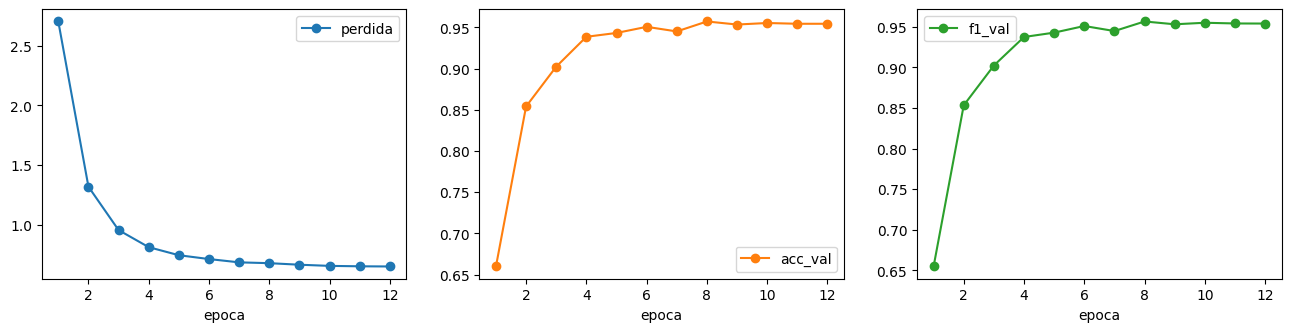
\includegraphics[width=0.9\textwidth]{curvas_entrenamiento.png}
\caption{Fine-tuning de ConvNeXt-Small: pérdida de entrenamiento, accuracy y F1 macro de validación por época.}
\label{fig:curvas}
\end{figure*}

En validación, el modelo A alcanzó un F1 macro de 0.978 y el modelo B, de 0.952. La Fig.~\ref{fig:peso} muestra el F1 de validación del ensemble en función del peso $w$. La curva tiene un máximo interior en $w=0.55$, con F1 de 0.986, mayor que con cualquiera de los dos modelos solos ($w=0$ o $w=1$). Esto confirma que ambos modelos se complementan.

\begin{figure}[!t]
\centering
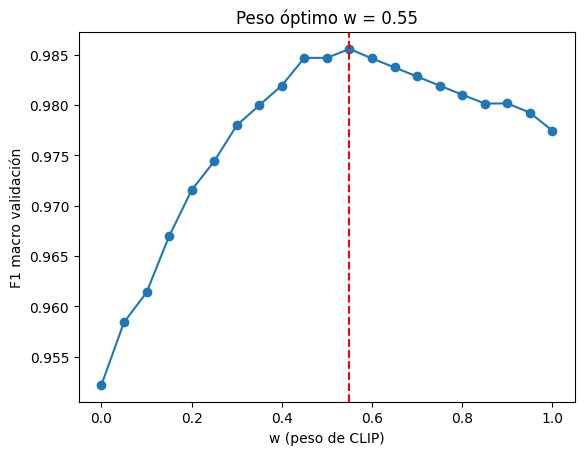
\includegraphics[width=0.8\columnwidth]{peso_ensemble.png}
\caption{F1 macro de validación del ensemble según el peso $w$ de CLIP. El óptimo es $w=0.55$.}
\label{fig:peso}
\end{figure}

\subsection{Evaluación en el conjunto de prueba}
\begin{figure*}[!t]
\centering
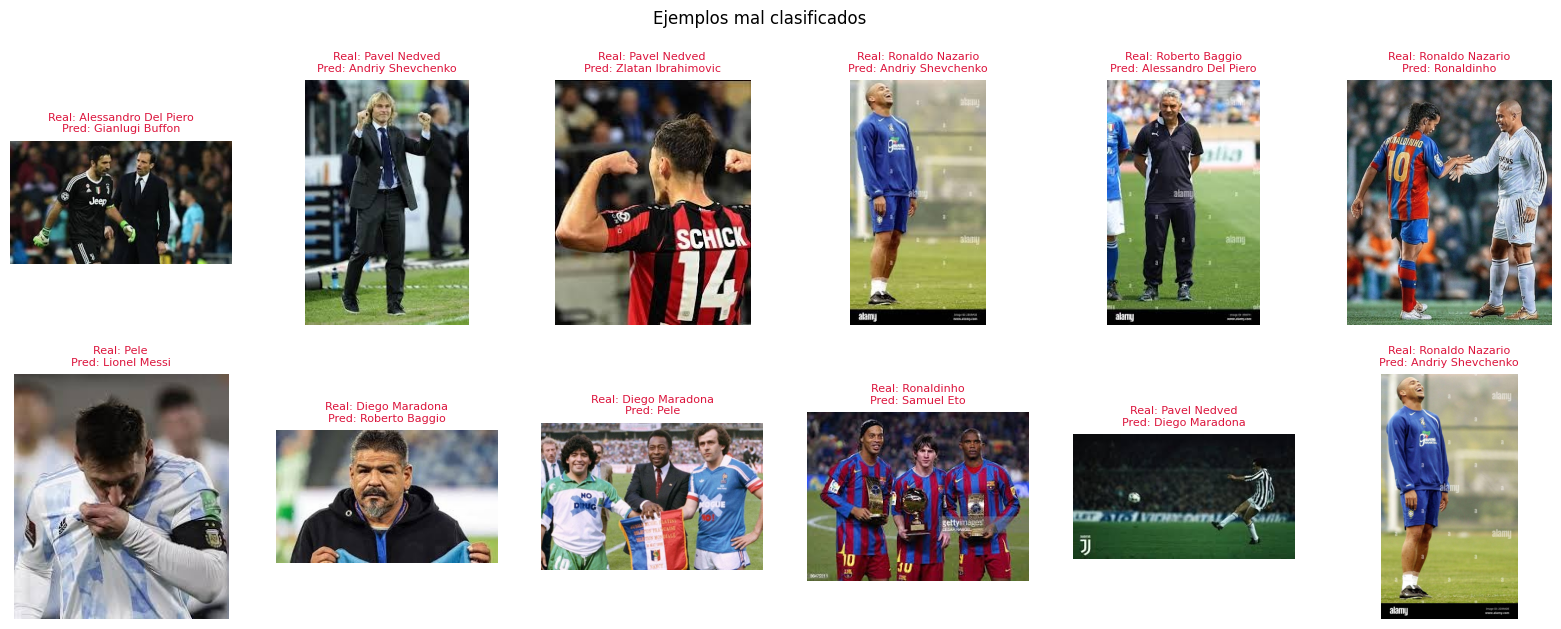
\includegraphics[width=0.85\textwidth]{errores.png}
\caption{Ejemplos de imágenes mal clasificadas por el ensemble (etiqueta real y predicha).}
\label{fig:errores}
\end{figure*}
La Tabla~\ref{tab:res} resume los resultados en las 1\,077 imágenes de prueba:
\begin{itemize}
\item CLIP \textit{zero-shot}, sin ningún entrenamiento, ya obtiene un F1 de 0.910. Esto indica que el modelo preentrenado ``conoce'' a estos jugadores.
\item El clasificador lineal sobre CLIP lo eleva a 0.959.
\item ConvNeXt afinada alcanza 0.934.
\item El ensemble obtiene los mejores valores en todas las métricas, con \textbf{recall macro de 0.968 y F1 macro de 0.968}. Comete 32 errores en 1\,077 imágenes, una tasa de error del 3\,\%.
\end{itemize}

\begin{table}[!t]
\centering
\caption{Métricas macro en el conjunto de prueba (1\,077 imágenes)}
\label{tab:res}
\footnotesize
\setlength{\tabcolsep}{4pt}
\begin{tabular}{lcccc}
\toprule
\textbf{Modelo} & \textbf{Acc.} & \textbf{Prec.} & \textbf{Recall} & \textbf{F1}\\
\midrule
CLIP \textit{zero-shot} (ref.) & 0.913 & 0.917 & 0.910 & 0.910\\
A. CLIP + Reg. logística & 0.961 & 0.960 & 0.959 & 0.959\\
B. ConvNeXt-Small & 0.936 & 0.937 & 0.933 & 0.934\\
\textbf{Ensemble ($w=0.55$)} & \textbf{0.970} & \textbf{0.970} & \textbf{0.968} & \textbf{0.968}\\
\midrule
Requisito & -- & -- & $>0.9$ & $>0.9$\\
\bottomrule
\end{tabular}
\end{table}

\subsection{Análisis por clase y errores}
La Tabla~\ref{tab:clases} muestra el \textit{recall} y el F1 por jugador, y la Fig.~\ref{fig:cm}, la matriz de confusión. Los resultados por clase son:
\begin{itemize}
\item Cinco jugadores se clasifican sin errores (F1 = 1.000): Iniesta, Cavani, Casillas, Modric y Salah.
\item Las clases más difíciles son Pavel Nedved (recall 0.889), Ronaldo Nazário (0.900), Pelé (0.917) y Maradona (0.918).
\end{itemize}
Estas cuatro clases coinciden con los jugadores que tienen menos imágenes y más fotografías antiguas o de baja calidad. Aun así, todas las clases superan 0.88 de \textit{recall} y 0.91 de F1.

La Fig.~\ref{fig:errores} muestra ejemplos mal clasificados. Los errores se concentran en tres tipos de imagen:
\begin{itemize}
\item Fotos con varios jugadores, donde el modelo identifica a otra persona de la escena.
\item Imágenes en las que el jugador aparece muy pequeño o de espaldas.
\item Fotografías en blanco y negro de jugadores de la misma época.
\end{itemize}
Por ejemplo, una imagen etiquetada como Maradona muestra juntos a Maradona, Pelé y Platini, y el modelo predice Pelé.

Además, algunos de los ``errores'' son en realidad etiquetas incorrectas del conjunto de datos. Una imagen etiquetada como Pelé muestra a Lionel Messi con la camiseta de Argentina, y el modelo predice correctamente Messi. Por lo tanto, el desempeño real del modelo es ligeramente superior al medido.

\begin{table}[!t]
\centering
\caption{Recall y F1 por clase del ensemble (prueba)}
\label{tab:clases}
\footnotesize
\setlength{\tabcolsep}{3pt}
\begin{tabular}{lcc|lcc}
\toprule
\textbf{Jugador} & \textbf{Rec.} & \textbf{F1} & \textbf{Jugador} & \textbf{Rec.} & \textbf{F1}\\
\midrule
Del Piero & 0.922 & 0.931 & Modric & 1.000 & 1.000\\
Iniesta & 1.000 & 1.000 & Salah & 1.000 & 1.000\\
Shevchenko & 0.981 & 0.962 & Nedved & 0.889 & 0.914\\
C. Ronaldo & 1.000 & 0.990 & Pelé & 0.917 & 0.930\\
Drogba & 0.980 & 0.990 & Giggs & 1.000 & 0.981\\
Maradona & 0.918 & 0.947 & Baggio & 0.939 & 0.939\\
Cavani & 1.000 & 1.000 & R. Carlos & 0.960 & 0.960\\
Totti & 1.000 & 0.990 & Ronaldinho & 0.979 & 0.949\\
Buffon & 0.981 & 0.981 & R. Nazário & 0.900 & 0.935\\
Casillas & 1.000 & 1.000 & Eto'o & 1.000 & 0.981\\
Messi & 0.940 & 0.940 & Ibrahimović & 0.981 & 0.981\\
\midrule
\multicolumn{3}{l}{\textbf{Promedio macro}} & & \textbf{0.968} & \textbf{0.968}\\
\bottomrule
\end{tabular}
\end{table}

\begin{figure}[!t]
\centering
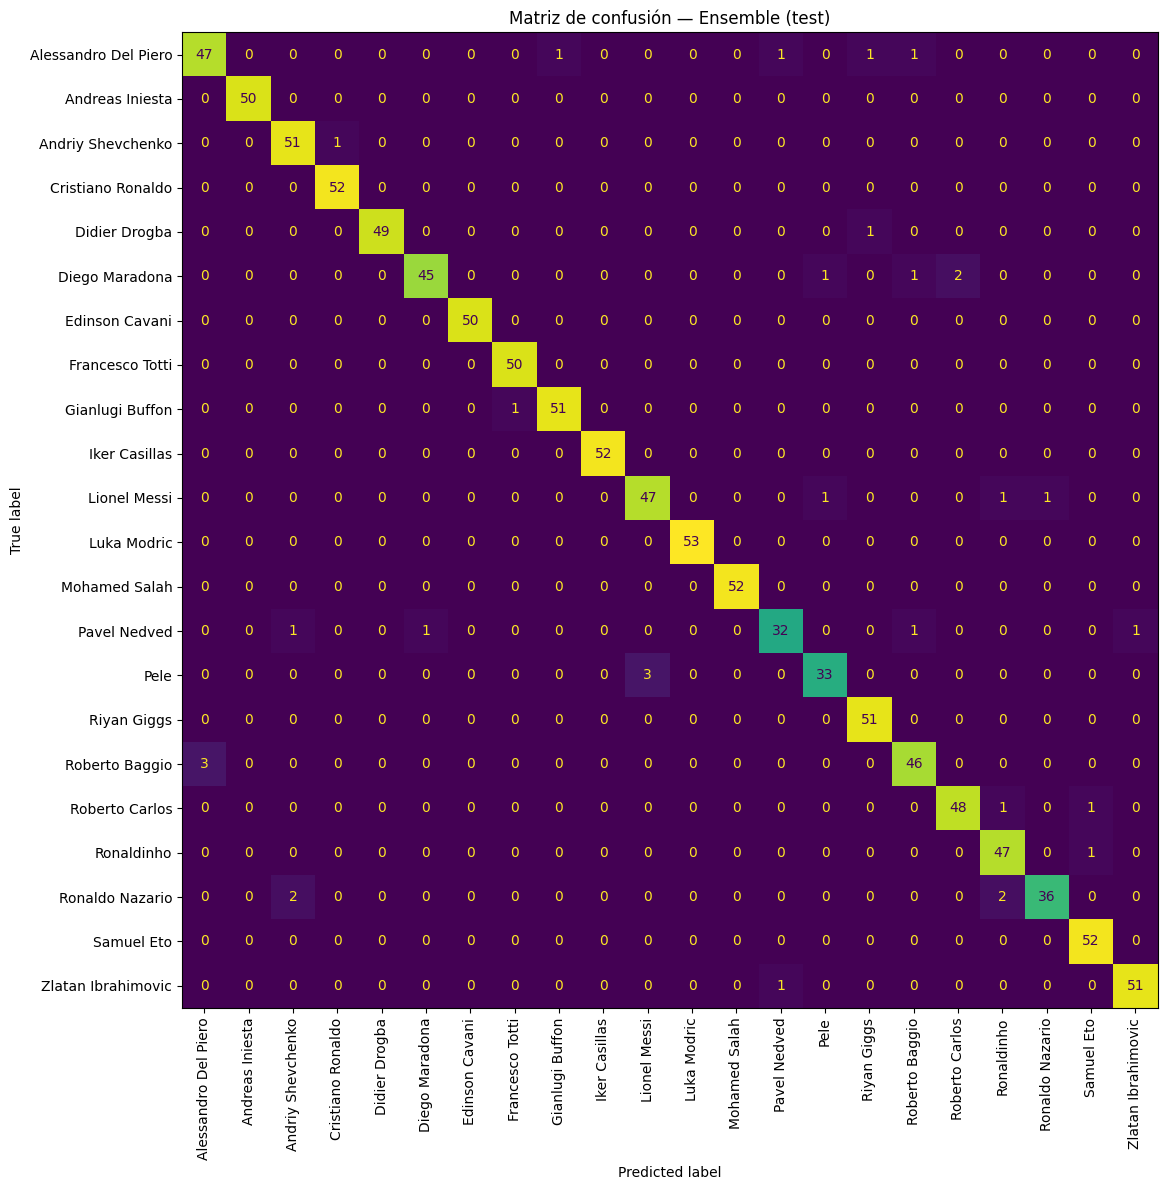
\includegraphics[width=\columnwidth]{matriz_confusion.png}
\caption{Matriz de confusión del ensemble en el conjunto de prueba.}
\label{fig:cm}
\end{figure}


\section{Discusión}
Los resultados muestran que, con alrededor de 300 imágenes por clase y condiciones muy variables, la calidad de las representaciones preentrenadas es el factor decisivo. CLIP, entrenado con pares imagen--texto de internet, aprendió asociaciones entre rostros, camisetas, escenarios y nombres de personas conocidas. Por eso basta un clasificador lineal sobre sus vectores para superar a una CNN reentrenada por completo.

Aun así, ConvNeXt aporta información complementaria: rasgos visuales finos aprendidos específicamente de este conjunto de datos. Gracias a ello, el ensemble reduce los errores de 42 (CLIP solo) a 32.

Este trabajo tiene dos limitaciones:
\begin{itemize}
\item \textbf{Fotos con varias personas:} el modelo clasifica la imagen completa. Un detector de rostros o de personas previo a la clasificación podría reducir esos errores.
\item \textbf{Origen de los datos:} las imágenes provienen de buscadores web, por lo que podrían existir casi-duplicados (misma foto recortada o redimensionada) que el hash MD5 no detecta.
\end{itemize}

\section{Conclusiones}
Se desarrolló un ensemble basado en \textit{transfer learning} para clasificar imágenes de 22 futbolistas. Combina CLIP ViT-L/14 con regresión logística y ConvNeXt-Small afinada mediante \textit{soft voting} ponderado.

En el conjunto de prueba el modelo obtiene un recall macro de 0.968 y un F1 macro de 0.968, por encima del requisito de 0.9, y supera a cada componente por separado. Las clases con menor desempeño son las de jugadores históricos con menos imágenes disponibles, lo que señala la cantidad y la calidad de los datos como la principal vía de mejora.

\begin{thebibliography}{9}
\bibitem{dataset} balabaskar, ``Golden Foot football players image dataset,'' Kaggle. [Online]. Available: \url{https://www.kaggle.com/datasets/balabaskar/golden-foot-football-players-image-dataset}
\bibitem{dietterich} T. G. Dietterich, ``Ensemble methods in machine learning,'' in \textit{Proc. Int. Workshop Multiple Classifier Systems}, 2000, pp. 1--15.
\bibitem{clip} A. Radford \textit{et al.}, ``Learning transferable visual models from natural language supervision,'' in \textit{Proc. ICML}, 2021, pp. 8748--8763.
\bibitem{vit} A. Dosovitskiy \textit{et al.}, ``An image is worth 16x16 words: Transformers for image recognition at scale,'' in \textit{Proc. ICLR}, 2021.
\bibitem{convnext} Z. Liu \textit{et al.}, ``A ConvNet for the 2020s,'' in \textit{Proc. IEEE/CVF CVPR}, 2022, pp. 11976--11986.
\bibitem{timm} R. Wightman, ``PyTorch image models,'' GitHub repository, 2019. [Online]. Available: \url{https://github.com/huggingface/pytorch-image-models}
\bibitem{adamw} I. Loshchilov and F. Hutter, ``Decoupled weight decay regularization,'' in \textit{Proc. ICLR}, 2019.
\bibitem{labelsmooth} C. Szegedy, V. Vanhoucke, S. Ioffe, J. Shlens, and Z. Wojna, ``Rethinking the inception architecture for computer vision,'' in \textit{Proc. IEEE CVPR}, 2016, pp. 2818--2826.
\end{thebibliography}

\end{document}
